






Os dados coletados forneceram uma base para as análises onde se verificou os pontos principais de cada técnica bem como a relação entre os modelos de extração de tópicos na seleção dos segmentos. Outros critérios podem ser levados em conta visto a subjetividade das avaliações bem como outros experimentos são necessários para obter melhores resultados.

averiguar o sistema na necessidade de análises mais profundas.































Nessa seção, os dados coletados das avaliações são apresentados e analisados. Os
modelos de extração de tópicos discutidos nesse trabalhos são comparados de acordo com
os critérios mencionados anteriormente: (1) comparar algoritmos de extração de tópicos na
tarefa de extração de padrões no contexto das atas de reunião, (2) analisar a qualidade dos
descritores extraídos para recuperar os documentos dos grupos. Além disso, as questões
referentes à segmentação, são analisadas a fim de validar a performance do segmentador
empregado, como complemento ao experimento discutido na Seção 4.











as questões referentes à segmentação foram apresentadas juntamente com as 





"No caso do KMeans a quantidade de usuários que identificaram que os descritores foram bons foi bem maior do que ... no caso do outro ... enfim" 


\textit{``Todos os trechos apresentados compartilham um mesmo assunto.''}
\textit{``As palavras \textit{<descritores>} resumem bem o assunto tratado nos trechos.''}
\textit{``Existem trechos que não tratam de um único assunto?''}
\textit{``Existem trechos incompletos e insuficientes para compreensão do assunto do trecho?''}






	\caption{Contagem de respostas referente a primeira questão cujo enunciado foi:\textit{``Todos os trechos apresentados compartilham um mesmo assunto.''}. O eixo vertical indica a frequência das alternativas representadas no eixo horizontal. }






	\caption{Contagem de respostas referente a primeira questão cujo enunciado foi:\textit{``Todos os trechos apresentados compartilham um mesmo assunto.''}. O eixo vertical indica a frequência das alternativas representadas no eixo horizontal por:
		a=\textit{``Discordo Totalmente''}
		b=\textit{``Discordo Parcialmente''}
		c=\textit{``Não Concordo, nem Discordo''}
		d=\textit{``Concordo Parcialmente''}
		e=\textit{``Concordo Totalmente''}.
	}



		\textit{``Discordo Totalmente''}
		\textit{``Discordo Parcialmente''}
		\textit{``Não Concordo, nem Discordo''}
		\textit{``Concordo Parcialmente''}
		\textit{``Concordo Totalmente''}.


		\textit{``Nenhum''};
		\textit{``Poucos''};
		\textit{``Nem muitos, nem poucos''};
		\textit{``Muitos''} e 
		\textit{``Todos''}.



% , conforme mostrado:
% 
% \begin{enumerate}
	% \item Todos os trechos apresentados compartilham um mesmo assunto.
	% \item As palavras \textit{<descritores>} resumem bem o assunto tratado nos trechos.
	% \item Existem trechos que não tratam de um único assunto?
	% \item Existem trechos incompletos e insuficientes para compreensão do assunto do trecho?
% \end{enumerate}
%


% o segmentador deve retornar trechos 
% ser suficientes para que o usuário compreenda o assunto 
% Nessa seção, os dados referentes à qualidade do segmentador são apresentados e analisados.
% Esse experimento foi aproveitado para validar o segmentador empregado nesse trabalho. 

a quantidade de usuários que concordam com a afirmação de que os termos são bons descritores foi bem maior em relação ao que discordam.

% a quantidade de usuários que reconhecem os termos como bons descritores foi bem maior que relação aos que os julgaram 

a maior diferença entre as opiniões positivas e negativas, sendo a maioria concordante com a afirmação de que os descritores extraídos são bons atributos para descrever o teor dos segmentos extraídos.






% --------------------------------------------------


Conforme as configurações, cada foi configurado para extrair 70 tópicos e selecionar 5 termos para descreve-los. 

O grupo selecionado pela busca é identificado pelos descritores .... e contem X segmentos.

Consulta 1 "compra de equipamentos"
	- K-Means 
		- Descritores "compra, material, verba, permanente e valor"
		- 13 Segmentos
	- LDA
		- Descritores "verba, compra, pagamento, material e valor"
		- 47 Segmentos
	- PLSA
		- Descritores "verba, compra, pagamento, valor e realizada"
		- 9 Segmentos

Consulta 2 "defesa de dissertação"
	- K-Means 
		- Descritores "orientada, meses, defesa, prazo e dissertação"
		- 12 Segmentos
	- LDA
		- Descritores "aprovado, defesa, pedido, dissertação e orientada"
		- 19 Segmentos
	- PLSA
		- Descritores "orientada, prazo, bolsa, meses e defesa"
		- 19 Segmentos

% --------------------------------------------------





% certa dificuldade em julgar capacidade dos descritores em representar bem o tópico.  
% valores entre 60 e 80 mostraram melhores resultados, 
% melhores resultados aparentes na visão de usuário.



Ao analisar os resultados do K-Means os avaliadores identificaram que, na maioria dos casos, houve resultados satisfatórios, principalmente quanto a representatividade dos descritores. Embora os avaliadores apontem imperfeições, esse modelo apresenta maior uniformidade em relação aos demais.


Com base em observações empíricas, verificou-se que valores entre 60 e 80 mostraram melhores resultados, em que valores abaixo de 60 Nesse trabalho, optou-se por configurar os algoritmos para extrair 70 tópicos da coleção de segmentos por apresentar melhores resultados aparentes na visão de usuário.



opiniões variam como esperado...
o que mais interessa?
--> podem ser considerados satisfatórios na tarefa de criar uma estrutura 

se os descritores são palavras que 
se os descritores são palavras que podem ser usadas como espaço de busca.



% a coesão dos segmentos em relação a semelhança dos segmentos em termos de assunto. 
% a qualidade de uma consulta à coleção de documentos a partir das técnicas de extração de tópicos analisadas nessa avaliação, ou seja, 
% dos segmentos retornados pelas técnicas de extração de tópicos, sendo que cada indivíduo analisou uma consulta à coleção de documentos com resultados das técnicas de extração de tópicos. 

% Os resultados desses cenários foram apresentados a um grupo de usuários que individualmente avaliaram a qualidade de uma consulta à coleção de documentos a partir das técnicas de extração de tópicos analisadas nessa avaliação, ou seja, cada indivíduo avaliou 3 cenários distintos, .
% Os resultados desses cenários foram apresentados a um grupo de usuários que individualmente avaliaram a qualidade dos segmentos retornados pelas técnicas de extração de tópicos, sendo que cada indivíduo analisou uma consulta à coleção de documentos com resultados das técnicas de extração de tópicos. 



Os resultados de cada cenário foram apresentados ao usuário que pode ler os segmentos retornados e expor sua percepção a cerca dos resultados.


 1 - Motivação para o experimento.
 2 - Escolha das questões.
 3 - Escolha dos participantes.
 4 - Procedimento (2 consultas, técnicas em ordens diferentes).
 5 - Medidas para avaliação.
 6 - Conclusão e discussão.


% Nesse trabalho, os algoritmos de extração de tópicos foram avaliados subjetivamente. 
 % Vale dizer que nessa avaliação o sistema de recuperação de informação não é analisado para que este não interfira na avaliação dos extratores, contudo, o sistema final poderá  ranquear também os segmentos com maior relevância de um ou mais tópicos por meio de técnicas de recuperação de informação. 
% Como já mencionado no Capítulo~\ref{sec:modulo-consulta} 
% Para cada cenário, resultou em uma lista de segmentos filtrados pela similaridade entre os descritores e a consulta.
% coletou-se aleatoriamente 
 % Nessa avaliação, devido a proximidade a técnica de segmentação textual também foi avaliada subjetivamente em complemento a análise estatística apresentada no Capítulo~\ref{cap-segmentadores}
% coletados foram analisados a fim de avaliar os algoritmos 
% A questão 1 está relacionada ao agrupamento dos segmentos. Pretende-se avaliar a Semelhança dos trechos em termos de assunto. O avaliador é questionado sobre 
% onde o avaliador indica o quanto os 
% enquanto a questão 4 refere-se a sua completude, 
% Referem-se à coesão de cada segmento e sua completude,respectivamente.
% a resposta diz respeito

% -? A Silueta já não é composta por coesão e separação?
% -> Como deve ser uma avaliação de extratores de tópicos? --> 

"Semelhança dos trechos em termos de assutno"

" Seleciona o tópico com maior relevância com a consulta "


% , em que o valor 70 mostrou 
% A fim de obter valores ótimos para esse parâmetro, realizou-se um teste prévio 
% Inicialmente, realizou-se um teste prévio a fim de obter valores ótimos para esse parâmetro pela analise das medidas Silhueta e Coesão. 
% e comparações
% com melhores resultados.  
% Optou-se por uma avaliação subjetiva 

% LDA - Gibbs Sampling
% Parâmetros 
	% Silueta e Coesão para o K-Means
	% Alpha e Beta do LDA
	% PLSA ???

% Durante os primeiros testes empíricos a qualidade dos resultados mostrou-se sensível à quantidade de tópicos extraídos, em que o valor 70 mostrou melhores resultados. Outro fator importante é a quantidade de descritores selecionados para cada tópico, com base no experimento de anotações em segmentação, os anotadores selecionaram em média 5 palavras para descrever os segmentos, sendo esse valor adotado para a avaliação.



% --> o processo de recuperação de informação filtrou um conjunto de segmentos. Dentre esses segmentos, 5 foram escolhidos aleatoriamente.




% - - - - - - - - - - - - - - - - - - - - - - - - - - - - - - 

Avaliação Subjetiva do extrator de tópicos:

(1) comparar algoritmos de extração de tópicos na tarefa de extração de padrões no contexto das atas de reunião, (2) analisar a qualidade dos agrupamentos no que tange a navegação por grupos com mesmo tópico, (3) analisar a qualidade dos descritores extraídos para recuperar os documentos dos grupos.


Tarefas:
Localizar segmentos que abordem esse assunto na lista ranqueada.
Localizar segmentos que abordem esse assunto utilizado o agrupamento.
Encontrar o documento original de um segmento que aborde esse assunto.

* É possível identificar claramente os tópicos das coleções com bases nas respectivas categorias?
* A navegação pelos tópicos ajuda a conduzir o usuário para o documento desejado?
* Os descritores dos tópicos são bons representantes do assunto dos documentos?
* Os segmentos apresentados são suficientes para entender o tópico?



 % ------------------------------

 - O K-Means se sobre-sai enquanto PLSA e LDA são equivalentes.

--> O segmentador, sendo uma etapa anterior a extração de tópicos, influencia na qualidade do grupos??

--> O K-means traz melhores segmentos (Sem misturar assuntos) em relação aos outros métodos.

'Aparentemente o K-means seleciona os trechos mais coesos, mas precisa de mais experimentos, mais amostras ...'


 1 - Motivação para o experimento.
 2 - Escolha das questões.
 3 - Escolha dos participantes.
 4 - Procedimento (2 consultas, técnicas em ordens diferentes).
 5 - Medidas para avaliação.
 6 - Conclusão e discussão.


% ------------------------------
% ------------------------------

--> Seria uma tecnica mais estável que outra? 


--> Com os meus avaliadores T1 > T2 > T3
--> Incluindo os da Katti   T1 > T2 = T3;
19:10 --> "Informação importante"
quantos da Consulta 1 e da 2
as localiazações
Afinidade -- quantificar
Procedimento --> Ordem alternada das Técnicas


% ------------------------------



'Usando o K-Means as pessoas identificaram que na maioria dos casos foi .. não é perfeito mais ... tem uma uniformidade maior em termos dos assuntos '


% Neste capítulo, o processo de extração de tópicos em segmentos de atas de reunião é avaliado. A avaliação experimental neste trabalho é focada em três pontos principais: (1) Comparar algoritmos de extração de tópicos na tarefa de extração de padrões no contexto das atas de reunião.  (2) Analisar a qualidade dos agrupamentos no que tange a navegação por grupos com mesmo tópico, (3) Analisar a qualidade dos descritores extraídos para recuperar os documentos dos grupos.  %(padrões = descritores e agrupamento)  



Nas próximas seções, são apresentadas as coleções textuais a serem utilizadas na avaliação experimental. Em seguida, é descrita a configuração dos experimentos, com o ajuste de parâmetros dos algoritmos e os critérios de avaliação. Por fim, são apresentados os experimentos realizados e uma análise dos resultados.


% --------------->>
Neste capítulo, o processo de extração de tópicos em sub-documentos de atas de reunião é avaliado. A avaliação experimental neste trabalho é focada em três pontos principais: 
(1) Analisar a qualidade dos agrupamentos no que tange a navegação por grupos com mesmo tópico, 
(2) Analisar a qualidade dos descritores extraídos para recuperar os documentos dos grupos.
% na representação dos sub-documentos.





1) Is it possible to identify clearly the topics of the collections
based on the respective categories?
2) Does the browsing through the topic hierarchy conduced
the user to a desired document set?
For both evaluations the used grades were:
0 - Nothing;
1 - Little;
2 - Fair;
3 - Good;
4 - Excellent


\item Os descritores dos tópicos são bons representantes do assunto dos documentos?
\item É possível indentificar claramente os 
\item A navegação pelos topicos ajuda a encontrar o assunto desejado?







% Nesse capítulo, as técnicas de extração de tópicos são analisadas em no que tange a qualidade dos agrupamentos e na capacidade dos descritores em representar os segmentos. 
%
% O objetivo é comparar algoritmos de extração de tópicos na tarefa de extração de padrões no contexto

% na capacidade dos descritores em representar os segmentos. 
%


\begin{figure}[!h] \centering     %%% not \center

	\subfigure{ \label{fig:seg1}
		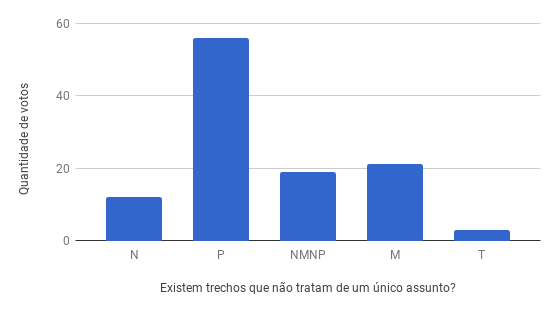
\includegraphics[width=.48\textwidth]{conteudo/capitulos/figs/figuras-experimento/Q3-Seg.png}
	}	
	\subfigure{ \label{fig:seg2}
		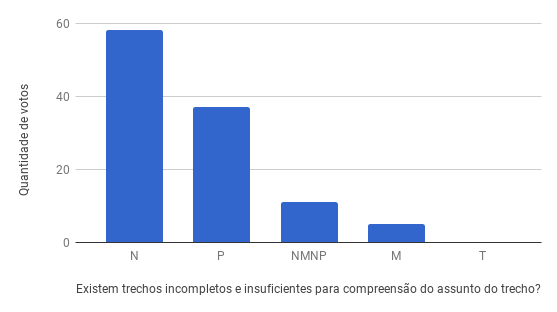
\includegraphics[width=.48\textwidth]{conteudo/capitulos/figs/figuras-experimento/Q4-Seg.png}
	}
	\caption{Contagem de respostas referente a terceira e quarta questão. Os eixos verticais indicam as frequências das alternativas representadas no eixos horizontais por:
		a=\textit{``Nenhum''}
		b=\textit{``Poucos''}
		c=\textit{``Nem Muitos, nem Poucos''}
		d=\textit{``Muitos''}
		e=\textit{``Todos''}.
	}
	\label{fig:Q3e4}
\end{figure}

\begin{figure}[!h] \centering     %%% not \center

	\subfigure{ \label{fig:seg1}
		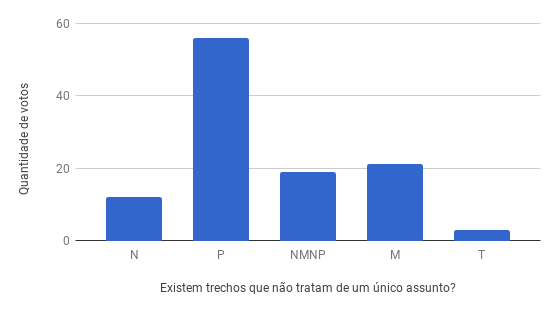
\includegraphics[width=.48\textwidth]{conteudo/capitulos/figs/figuras-experimento/Q3-Seg.png}
	}	
	\subfigure{ \label{fig:seg2}
		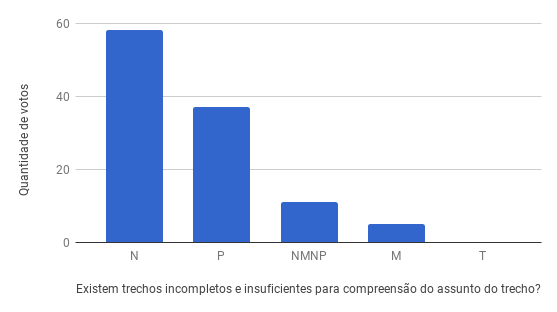
\includegraphics[width=.48\textwidth]{conteudo/capitulos/figs/figuras-experimento/Q4-Seg.png}
	}
	\caption{Contagem de respostas referente a quarta questão em que o eixo vertical indica a frequência das alternativas.  }
	\label{fig:Q3}
\end{figure}

% Na linha superior observa-se os resultados a terceira questão, 

% e na inferior, os resultados da quarta questão, 
